\documentclass[a4paper,10pt]{article}

\usepackage{tikz}
\usepackage{fullpage}
\usepackage{amsmath,amsthm,amsfonts,amssymb,amscd}
\usepackage{mathtools}
\usepackage{colortbl}
\usepackage{xcolor}
\usepackage{graphicx}
\usepackage{titlesec}
\usepackage{xepersian}
\usepackage{multirow}
\usepackage{caption}
\usepackage{fancyhdr}
\usepackage{mdframed}


% ---------------------------
%      Color Palette
% ---------------------------
%\definecolor{BgDark}{HTML}{F5F7FF}      % page background
%\definecolor{BgCard}{HTML}{EDEFF7}      % card / panel background
%\definecolor{AccentBlue}{HTML}{3A5CCC}
%\definecolor{AccentPurple}{HTML}{7C5ACF}
%\definecolor{AccentCyan}{HTML}{2FA4B7}
%\definecolor{AccentGold}{HTML}{B5892D}
%\definecolor{TextPrimary}{HTML}{1F2335}
%\definecolor{TextMuted}{HTML}{6B7089}
%\definecolor{RuleLine}{HTML}{D6D9E6}
%
%\pagecolor{BgDark}
%\color{TextPrimary}

\definecolor{BgDark}{HTML}{141420}
\definecolor{BgCard}{HTML}{1E1E2E}
\definecolor{AccentBlue}{HTML}{7AA2F7}
\definecolor{AccentPurple}{HTML}{BB9AF7}
\definecolor{AccentCyan}{HTML}{7AA2F7}
\definecolor{AccentGold}{HTML}{E0AF68}
\definecolor{TextPrimary}{HTML}{CDD6F4}
\definecolor{TextMuted}{HTML}{6C7086}
\definecolor{RuleLine}{HTML}{313244}

\pagecolor{BgDark}
\color{TextPrimary}

% ---------------------------
%  RTL-safe Info Box
% ---------------------------
\newmdenv[
backgroundcolor=BgCard,
fontcolor=TextPrimary,
linecolor=AccentBlue,
linewidth=1.2pt,
rightline=true,   % RTL: accent border on the RIGHT
leftline=false,
topline=false,
bottomline=false,
innerrightmargin=12pt,
innerleftmargin=12pt,
innertopmargin=10pt,
innerbottommargin=10pt,
skipabove=10pt,
skipbelow=10pt,
]{infobox}
% ---------------------------
%        Font Setup
% ---------------------------
\settextfont{Vazir.ttf}[
    BoldFont = Vazir-Bold.ttf,
    Path = fonts/
]
\setlatintextfont{Vazir.ttf}[
    BoldFont = Vazir-Bold.ttf,
    Path = fonts/
]

% ---------------------------
%     Custom Adjustments
% ---------------------------
\renewcommand{\baselinestretch}{1.2}
\renewcommand{\thesection}{\arabic{section}}
\newcommand{\GroupA}{\noindent \textcolor{AccentGold}{گروه \lr{a}}}
\newcommand{\GroupB}{\noindent\textcolor{AccentCyan}{گروه \lr{b}}}

% User-defined commands for homework info (adjust as needed)
\newcommand{\HomeworkNumber}{1}
\newcommand{\HomeworkDeadline}{1403/12/22}
\newcommand{\id}{\texttt{\detokenize{@Amir_Hossein_Afshar}}}



\begin{document}

% header
\begin{infobox}

\begin{minipage}{0.295\textwidth}
	\raggedleft
	مبانی هوش مصنوعی \\
	دانشگاه فردوسی مشهد\\
	گروه مهندسی کامپیوتر
\end{minipage}
\begin{minipage}{0.4\textwidth} 
	\centering 
	
\includegraphics[scale=0.3]{assets/fum-logo.png}
\end{minipage}
\begin{minipage}{0.295\textwidth}
	آزمون میانترم جبرانی \\
	مورخ 30 خرداد 1405 \\
	مدت زمان آزمون: 60 دقیقه
\end{minipage}
\end{infobox}


\begin{infobox}
	دانشجویان محترم لطفا به موارد زیر توجه فرمایید:
	\begin{itemize}
		\itemsep0.4em
		\item
		تحویل آزمون فقط از طریق سامانه آموزش مجازی دانشگاه امکان‌پذیر است.
		\item
		پاسخ آزمون باید دست‌نویس، خوانا و با استفاده از خودکار آبی یا مشکی و یا به صورت دیجیتالی با استفاده از قلم نوری نوشته شوند و هرگونه پاسخ تایپی غیرقابل پذیرش است.
		\item
		از پاسخ حل‌شده دیگران استفاده نکنید. پیامدهای این کار با دانشجو می‌باشد.
		\item
		نوشتن جواب آخر به تنهایی نمره‌ای نداشته و تمام مراحل حل، مشمول نمره می‌باشد.
		\item
		در حل سوالات مدیریت زمان داشته باشید. زمان آزمون تمدید نخواهد شد. همچنین بدیهی است که ارسال پس از موعد، شامل نمره نخواهد بود.
		\item 
		فایل نهایی پاسخ به صورت pdf و نحوه نام‌گذاری فایل پاسخ مطابق جدول زیر باشد.
		
	\end{itemize}
	
	
	\vspace{2pt}
	
	% RTL-safe table: use center environment, manual column colors
	\begin{center}
		\arrayrulecolor{RuleLine}
		\begin{tabular}{|>{\columncolor{BgCard}\centering\arraybackslash}p{3cm}|>{\columncolor{BgDark}\centering\arraybackslash}p{7cm}|}
			\hline
			\textcolor{AccentCyan}{\bfseries\lr{Format}} &
			\texttt{\lr{StudentID-Full\_Name-midterm1.pdf}} \\
			\hline
			\textcolor{AccentGold}{\bfseries\lr{Example}} &
			\textcolor{TextMuted}{\texttt{\lr{9876543210-Alan\_Turing-midterm1.pdf}}} \\
			\hline
		\end{tabular}
		\label{tab:file_format}
	\end{center}
	
\end{infobox}


\vspace{2pt}
\textcolor{AccentCyan}{\rule{\linewidth}{0.8pt}}
% ---------------------------------
%          questions
% ---------------------------------
%%%%%%%%%%%%%%%%%%%%%%%%%%%%%%%%%%%%%%%%%%%%%%%%%%%%%%%%%%%%%%%%%%%%%%%%%%%%%%%%%%%%%%%%%%%%%%
\section{\textcolor{AccentGold}{سوال اول}}
به موارد زیر پاسخ دهید.
\begin{itemize}
	\item الف)
محدودیت زمان و حافظه از دلایل اصلی استفاده از توابع \lr{heuristic} و متوقف کردن جست‌وجو قبل از بررسی تمامی حالات می‌باشد. در به‌کارگیری روش دوم، دو مسئله \lr{non-quiescent positions} و \lr{horizon effect} به‌وجود می‌آیند. این مسائل را تعریف کنید.
\item ب)
توضیح دهید که ترتیب بازدید گره‌ها چه تاثیری بر عملکرد \lr{alpha-beta pruning} دارد. آیا در صورتی که این ترتیب کاملاً مطلوب باشد استفاده از \lr{alpha-beta pruning} منطقی است؟ جست‌وجو چطور؟ چرا؟
\end{itemize}
\textcolor{AccentCyan}{\rule{\linewidth}{0.4pt}}
%%%%%%%%%%%%%%%%%%%%%%%%%%%%%%%%%%%%%%%%%%%%%%%%%%%%%%%%%%%%%%%%%%%%%%%%%%%%%%%%%%%%%%%%%%%%%%
\section{\textcolor{AccentGold}{سوال دوم}}
	\begin{infobox}
	\textbf{صورت مسئله:} 
	در یک خط تولید پیشرفته صنعتی، مجموعه‌ای از $N$ فرآیند تولیدی باید به ترتیب برای تولید یک محصول نهایی پیچیده اجرا شوند. هر حالت $n$ در فضای جستجو، نشان‌دهنده مجموعه‌ای از فرآیندهای تکمیل‌شده است. هزینه انتقال از یک حالت به حالت بعدی، برابر با «میزان مصرف انرژی کوره مرکزی و استهلاک تجهیزات» بر حسب واحد زمان است. هدف، رسیدن به حالت پایانی (تکمیل تمام فرآیندها) با کمترین هزینه عملیاتی است.
\end{infobox}

\pagebreak
\noindent \textbf{محدودیت‌های حاکم بر خط تولید و ترتیب فرآیندها:}
\begin{enumerate}
	\item \textbf{$C_1$ (ترتیب و پیش‌نیازی):} برخی از فرآیندها دارای وابستگی شدید جفت‌جویی هستند؛ به این معنی که فرآیند $B$ دقیقاً و بدون هیچ فاصله‌ای باید بلافاصله پس از فرآیند $A$ اجرا شود، در غیر این صورت قطعه اولیه فاسد می‌شود.
	\item \textbf{$C_2$ (محدودیت منابع مشترک):} سه فرآیند کلیدی خط تولید نیاز به یک بازوی رباتیک مشترک دارند. بنابراین، این سه فرآیند به هیچ عنوان نمی‌توانند به صورت همزمان یا در بازه‌های متداخل پردازش شوند و باید کاملاً \lr{Sequential} زمانبندی شوند.
	\item \textbf{$C_3$ (پیکربندی مجدد):} هر بار که سیستم از یک نوع فرآیند (مثلاً قالب‌گیری) به نوع دیگر (مثلاً رنگ‌آمیزی) سوئیچ می‌کند، نیاز به ۱ گام زمانی برای کالیبراسیون و خنک‌سازی دستگاه‌ها دارد که هزینه ثابتی به سیستم تحمیل می‌کند.
\end{enumerate}

\begin{itemize}
	\item[\textbf{الف)}] 
	با استفاده از مفهوم \lr{Relaxation}، دو تابع هیوتیستیک متفاوت ($h_1$ و $h_2$) برای تخمین هزینه باقی‌مانده تا اتمام فرآیندها طراحی کنید:
	\begin{itemize}
		\item برای ساخت $h_1$ حداقل \textbf{دو مورد} از محدودیت‌های عملیاتی بالا ($C_1$ تا $C_3$) را \lr{Relax} کنید.
		\item برای ساخت $h_2$ \textbf{فقط یک مورد} از محدودیت‌ها را حذف کنید، به طوری که تابع $h_2$ نسبت به $h_1$ واجد ویژگی \lr{Informative} باشد و تخمین دقیق‌تر و بزرگ‌تری از هزینه واقعی ارائه دهد.
	\end{itemize}
	\textbf{منطق عملکردی و فرمول ریاضی} هر دو تابع هیوتیستیک پیشنهادی خود را به طور کامل تشریح کنید.
	
	\vspace{0.3cm}
	\item[\textbf{ب)}] 
	مفهوم \lr{Dominance} را بین این دو تابع هیوتیستیک تحلیل کنید. استفاده از کدام‌یک در الگوریتم $A^*$ فضای حالت را بیشتر \textbf{هرس} می‌کند و چرا؟ تعداد گره‌های تولید شده را در دو حالت به صورت کیفی مقایسه کنید.
	
	\vspace{0.3cm}
	\item[\textbf{ج)}] 
	آیا هیوتیستیک $h_2$ طراحی‌شده توسط شما، ویژگی \lr{Consistency} را در گراف تغییرات خط تولید ارضا می‌کند؟ با استفاده از رابطه مثلثی زیر، پاسخ خود را به صورت دقیق اثبات کنید یا یک توالی فرآیند کوچک به عنوان مثال نقض ارائه دهید:
	$$h(n) \le c(n, a, n') + h(n')$$
	
\end{itemize}
\textcolor{AccentCyan}{\rule{\linewidth}{0.4pt}}
%%%%%%%%%%%%%%%%%%%%%%%%%%%%%%%%%%%%%%%%%%%%%%%%%%%%%%%%%%%%%%%%%%%%%%%%%%%%%%%%%%%%%%%%%%%%%%
\section{\textcolor{AccentGold}{سوال سوم}}

درستی یا نادرستی گزاره‌های زیر را اثبات کنید:
\begin{latin}
\begin{enumerate}
	\item ${(A \to B) \land (\neg A \to C) \land (B \lor C \to D) \models D}$
	\item ${(A \lor B) \land (\neg A \lor C) \land (\neg B \lor D) \land (\neg C \lor G) \land (\neg D \lor G) \models G}$
	\item ${A \land (A \to B) \land ((A \to B) \to (B \to C)) \models C}$
	\item ${\neg A \land (A \to B) \models \neg B}$
\end{enumerate}
\end{latin}

\textcolor{AccentCyan}{\rule{\linewidth}{0.4pt}}
%%%%%%%%%%%%%%%%%%%%%%%%%%%%%%%%%%%%%%%%%%%%%%%%%%%%%%%%%%%%%%%%%%%%%%%%%%%%%%%%%%%%%%%%%%%%%%

\pagebreak
\section{\textcolor{AccentGold}{سوال چهارم}}
 در یک جدول متقاطع  متشکل از خانه های مسدود و غیرمسدود است که همچنین یک لیست از لغات نیز دارد. هدف ما این است که به هر خانه غیرمسدود یک حرف اختصاصدهیم به گونه ای که هر قطعه ی پیوسته از 
خانه های غیرمسدود که به صورت افقی یا عمودی کنار هم قرار گرفته اند، یک کلمه ی معتبر از فرهنگ لغت را تشکیل دهد. 
مثالی از یک جدول کلمات متقاطع حل شده در ادامه آمده است: 

\begin{figure}[h]
	\centering
	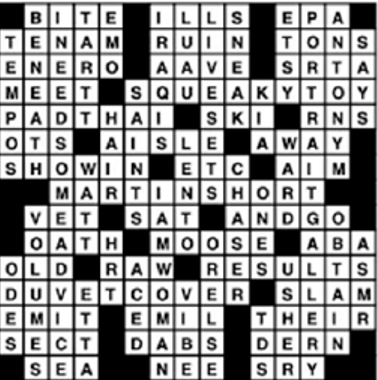
\includegraphics[scale=0.60]{assets/1.png}
\end{figure}

این مسئله را به عنوان یک مسئله ی ارضای محدودیت فرموله و مدلسازی کنید و 
متغیرها، دامنه ها و محدودیت ها به شکل کامل و دقیق مشخص کنید



\bigskip
\textcolor{AccentCyan}{\rule{\linewidth}{0.4pt}}



\end{document}
